
%%%%%%%%%%%%%%%%%%%%%%% file typeinst.tex %%%%%%%%%%%%%%%%%%%%%%%%%
%
% This is the LaTeX source for the instructions to authors using
% the LaTeX document class 'llncs.cls' for contributions to
% the Lecture Notes in Computer Sciences series.
% http://www.springer.com/lncs       Springer Heidelberg 2006/05/04
%
% It may be used as a template for your own input - copy it
% to a new file with a new name and use it as the basis
% for your article.
%
% NB: the document class 'llncs' has its own and detailed documentation, see
% ftp://ftp.springer.de/data/pubftp/pub/tex/latex/llncs/latex2e/llncsdoc.pdf
%
%%%%%%%%%%%%%%%%%%%%%%%%%%%%%%%%%%%%%%%%%%%%%%%%%%%%%%%%%%%%%%%%%%%
\documentclass{llncs}

\usepackage{amsmath, amsfonts, amssymb}
\usepackage{graphicx}
\usepackage{url}
\usepackage{blindtext}
\usepackage{enumitem}
\usepackage{graphicx}
\usepackage{amssymb}
\usepackage{amsmath}
\usepackage{algpseudocode}
\usepackage{caption}
\usepackage{subfig}
\usepackage{cite}
\usepackage{hhline}
\usepackage{authblk}
\usepackage{comment}
\usepackage[export]{adjustbox}

%\urldef{\mailsa}\path|{*********************}|
%\newcommand{\keywords}[1]{\par\addvspace\baselineskip
%\noindent\keywordname\enspace\ignorespaces#1}

\begin{document}

\mainmatter  % start of an individual contribution


\title{Geodesic Shape Regression of Continuous Medial Representation}
\author{No Author Given}
\institute{No Institute Given}

\maketitle

\begin{abstract}
Longitudinal shape analysis has shown great potential to improve our understanding of subject-specific changes of anatomy over time, 
in order to capture progression of disease or efficacy of therapy from baseline to follow-up observations. 
Shape regression estimates a continuous trajectory of shapes as the trend of time-discrete anatomical surfaces with the goal to quantify locality and magnitude of temporal changes. 
Such analysis traditionally requires appropriate choices for alignment and normalization of shapes, 
and therefore results are dependent on the type of alignment.
As an alternative, we model several shapes jointly as a multi-object complex to overcome the need for individual shape alignment, 
and to incorporate extrinsic pose changes caused by neighboring structures. 
Shapes in our work are continuous medial representations (CM-Reps), 
which capture intrinsic shape properties, such as local thickness, which are invariant to pose variations. 
Regression is represented by a geodesic flow of diffeomorphisms in the large deformation diffeomorphic metric mapping (LDDMM) framework which act on medial surfaces to produce continuously evolving CM-Reps. 
In contrast to existing methods, our model captures extrinsic shape changes via ambient space deformations as well as intrinsic shape changes encoded by the CM-Reps. 
Furthermore, our method provides explicit correspondence over the flow of CM-Reps, 
allowing us to accurately track local thickness measurements over time. 
We propose an optimization method that estimates a continuous trajectory of CM-Reps to match reconstructed shapes with observed shapes by a gradient descent scheme. 
To demonstrate stability and feasibility of the proposed method, we provide experimental validation on synthetic and real anatomical shape complexes.
%\keywords{Longitudinal Shape Analysis, Shape Regression, Medial Representation, 4D Skeleton}
\end{abstract}

\section{Introduction}

The study of anatomical shape change over time has drawn more attention recently through increased availability of repeated longitudinal scans of individual subjects and has shown great potential to improve our understanding of changes of anatomy related with disease progression~\cite{Gerig2016}. %Shape regression is an important tool for longitudinal shape analysis since it estimates a continuous shape change over time via modeling from a small number of scans distributed in time. Similar to traditional data regression methods, shape regression requires a model to represent shape changes and a metric to measure marginal error between the estimated model and observed shapes. 
%Longitudinal shape analysis considers possible temporal correlation between shapes from a same subject as a set and tracks shape changes of the set of shapes while shapes are considered as independent data in traditional shape analysis [].
%Longitudinal shape analysis has shown great potential to improve our understanding of subject-specific changes of anatomy over time, in order to capture progression of disease of efficacy of therapy from baseline to follow-up observations. 
% Previous studies suggested different models and metrics to model the shape changes over time with given observations.
Shape analysis is traditionally performed on a single structure and made invariant to pose by an alignment procedure, commonly Procrustes alignment. Invariance can also be achieved through the construction of equivalence classes, as with Kendall shape space~\cite{kendall84BLMS}. Statistical techniques have been developed to properly account for the non-linearity of the space~\cite{journals/ijcv/Fletcher13, fletcher2004principal}. Analysis of this type suffer from two main limitations. First, the resulting patterns of shape change are heavily influenced by initial alignment. Second, the analysis of an isolated and normalized anatomical structure doesn't account for external structural changes due to adjacent objects, e.g. the basal ganglia are pushed outward by the expansion of the lateral ventricles. 

One alternative to analyzing single shapes in isolation is regression analysis on full image volumes, which overcomes the need for object specific alignment and incorporates multiple structures~\cite{niethammer_geodesic, singh2015splines}. However, in many cases, there is not adequate contrast to accurately model small scale changes, or to capture changes to structures whose boundaries are fuzzy or obscured by partial voluming. In the case of poor contrast, image regression models may be improved by including shape priors in model estimation~\cite{SCI:Fis2014a}.

To address the importance of including multiple sources of geometry as a multi-object complex, ambient space regression methods have been proposed. These methods are based in the large deformation setting (LDDMM), where several sources and types of geometry contribute to the estimation of a single time-varying deformation of the ambient space~\cite{Rekik2016, Fishbaugh2013}. While ambient space methods account for interactions between neighboring structures, the momenta vectors which parameterize shape changes do not readily differentiate between extrinsic changes in pose and intrinsic changes to shape geometry. Extrinsic and intrinsic changes are coupled and it is not clear how to separate the two.

Decoupling extrinsic and intrinsic shape properties has been widely studied by skeletonization methods in image processing and graphics~\cite{Taglia2016}. Medial surfaces in~\cite{Siddiqi2002} capture intrinsic shape properties, however, statistical analysis is not straightfoward since correspondence between medial surfaces and shape boundaries are not established. Furthermore, different medial surfaces might have different topological properties, making correspondence impossible. Medial surfaces in~\cite{Pizer2003} aid statistical analysis on intrinsic shape properties since medial representations are in correspondence by a fixed graph. The continuous medial representation (CM-Rep)~\cite{Yushkevich2006} deforms a template CM-Rep and updates its attached radius scalar field to match a target shape. However, no previous skeletonization study has been suggested, in our knowledge, to estimate continuous or temporally correlated medial representations, which is of great interest to longitudinal shape analysis.

In this paper, we propose geodesic shape regression of CM-Reps to estimate a continuous and differentiable shape trajectory from intermittent observations. The proposed method estimates a model of continuous change of CM-Reps over time in the LDDMM setting by matching reconstructed shape boundaries of CM-Reps to observed shapes. As an outcome of the proposed method, we obtain the continuous trajectory of CM-Reps as well as their reconstructed shape boundary, capturing intrinsic as well as extrinsic shape properties in a single model. Thus, the proposed method estimates not only a continuous trajectory of shapes as suggested in previous literature, but it also estimates a spatiotemporal trajectory of medial surfaces which has not been reported before in our knowledge. Such a trajectory allows for the accurate tracking of local thickness measurements across time.

\section{Methods}

The proposed method estimates a continuous trajectory of medial surfaces and reconstructed shape boundaries over time. 
We begin with introducing the CM-Rep as a shape representation of medial surfaces of the suggested shape regression framework and describe how we estimate the continuous trajectories in LDDMM paradigm by matching reconstructed shape boundaries of CM-Reps to observation shapes. 

\subsection{Continuous Medial Representations}
\label{ssec:CMRep}

In this section, we will describe how shape are represented in our method with CM-Rep~\cite{Yushkevich2009}. 
CM-Rep, $\mathbf{m}$, is a parameterized continuous surface with radius scalar field $\mathbf{R}$ encoded on the surface. 
A shape boundary, $\mathbf{X}$, of $\mathbf{m}$ is reconstructed by maximum inscribed ball (MIB) with radius $\mathbf{R}$. 
Since $\mathbf{X}$ is a reconstructed shape from a medial surface $\mathbf{m}$, $\mathbf{X}^{\pm}(u)$ of $\mathbf{X}$ on opposite sides of $\mathbf{m}(u)$ 
can be described as the point of tangency between $\mathbf{X}(u)$ and MIB of $\mathbf{m}(u)$ and $\mathbf{R}(u)$, 
\begin{equation}
 \mathbf{X}^{\pm}(u) = \mathbf{m}(u) + \mathbf{R}(u)\mathbf{U}^{\pm}(u) \\
\end{equation}
where $u$ represents a parameter of $\mathbf{m}$ and $\mathbf{U}^{\pm}$ is the unit outward normal vectors on both directions to $\mathbf{X}$,
\begin{equation}
 \mathbf{U}^{\pm} = -\nabla_\mathbf{m} \mathbf{R} \pm \sqrt{ 1 - || \nabla_\mathbf{m} \mathbf{R} ||^2 }\mathbf{N}_\mathbf{m}.
\end{equation}
The CM-Rep $\mathbf{m}$ is represented as a surface triangular mesh with a fixed number of vertices. 
The edge information of the reconstructed shape $\mathbf{X}$ is copied from $\mathbf{m}$ on both sides of $\mathbf{X}^\pm$ to create a surface mesh of $\mathbf{X}$. 
This will guarantee that the surface mesh of $\mathbf{X}$ is well-defined from the well-defined medial surface mesh. 
Since the deformation flow $\mathbf{m}$ over time in our shape regression method is defined as a flow of diffeomorphisms, the reconstructed surface mesh stays as the well-defined surface mesh, which is important for our shape matching energy function. 

\subsection{Geodesic Shape Regression via Continuous Medial Representations}
\label{ssec:Regression}

To estimate a continuous trajectory of CM-Reps and shape boundaries, the method iterates between CM-Rep trajectory estimation with a fixed radius scalar field and radius scalar field estimation with a fixed CM-Reps at the time point of observation shapes. In the iteration process, the method matches a reconstructed shape boundary of CM-Rep to observation shapes by updating the geometry of CM-Reps and their radius scalar fields.

\subsubsection{Initialization}
The model requires an initial baseline CM-Rep to start with as a template $\mathbf{m}_0$ and initial radius scalar fields $\mathbf{R}_{t_i}$ at each observation time point. 
We initialize an initial baseline CM-Rep $\mathbf{m}_0$ by estimating a CM-Rep with the method suggested in~\cite{Yushkevich2009} at the first observation shape $\mathbf{O}_{t_0}$.
At each time point $t_i$, $R_{t_i}$ is estimated by the same method with an initial baseline CM-Rep $\mathbf{m}_0$. We only use $\mathbf{R}_{t_i}$ as initial radius scalar fields for our framework to estimate a continuous deformation over time of $\mathbf{m}_0$.

\subsubsection{CM-Rep Shape Trajectory Estimation}
\label{sssec:GeoUpdate}

The model estimates a diffeomorphic shape  trajectory of CM-Rep $\mathbf{m}$ from a set of observed shapes $\mathbf{O}_{t_i}$ with a fixed radius scalar field at each time point $\mathbf{R}_{t_i}$.
The geodesic flow of diffeomorphisms along with continuous time $t$, $\phi_t$ is estimated on control points $\mathbf{c}$ and momenta $\mathbf{\alpha}$ on $\mathbf{c}$~\cite{Fishbaugh2013}.
The method optimizes the energy function which measures the distance between a reconstructed shape boundary $\mathbf{X}_{t_i}$ from a fixed radius scalar field $\mathbf{R}_{t_i}$ and a deformed CM-Rep  $\phi_{t_i}( \mathbf{m}_0 )$ at time point $t_i$. 
\begin{equation}
 E( \mathbf{m}_0, \phi_t ) = \sum_{i=1}^{N_{obs}} || \mathbf{X}_{t_i} ( \phi_{t_i} (\mathbf{m}_0), \mathbf{R}_{t_i} ) - \mathbf{O}_{t_i} ||^2_{\mathit{W}*} + Reg( \phi_t ),
\end{equation}
where $Reg(\phi_t)$ is the regularity term of $\phi_t$ and $||\cdot||_{\mathit{W}*}^2$ is a shape distance defined as a varifold metric between meshes $\mathbf{X}_{t_i}$ and $\mathbf{O}_{t_i}$.
As discussed in Section~\ref{ssec:CMRep}, the reconstructed shape mesh $\mathbf{X}_{t_i}$ is well-defined and the surface normals are aligned as outward normal vectors from $\mathbf{m}$. 
However, the varifold metric suits well to our problem since the surface mesh of observed shape might have flipped normals and the correspondence between $\mathbf{O}_{t_i}$ and $\mathbf{X}_{t_i}$ are not defined. 

\subsubsection{Radius Scalar Field Estimation}
\label{sssec:RadUpdate}

We follow the radius scalar field estimation by solving biharmonic PDE to satisfy the sufficient conditions of valid inverse skeletonization suggested in~\cite{Yushkevich2009}.
The radius scalar field $\mathbf{R}$ is solved by biharmonic PDE with a potential function $\rho$ defined on $\mathbf{m}$ and boundary condition function $\tau$ on a fixed $\mathbf{m}$,

\begin{align}
 &\Delta_{\mathbf{m}}^2 f(\mathbf{R}) = \rho \\
 &f(\mathbf{R}) \|_{\gamma} = \tau^2 \\
 &f(\mathbf{R}), \nu \|_\gamma = -2 \tau \sqrt{ 1 - ( \frac{d\tau}{ds} ) } 
\label{eq:BiPDE}
\end{align}

where $f(\mathbf{R}) = \mathbf{R}^2$, the boundary condition function $\tau$ is a radius on the boundary of $\mathbf{m}$, $\Delta_{\mathbf{m}}$ denotes the Laplace-Beltrami operator on $\mathbf{m}$, $\gamma$ is the parameterized edge of $\mathbf{m}$ by the arc length $s$, and $f(\mathbf{R}), \nu$ denotes the gradient of $f$ with respect to the unit outward normal vector $\nu$. 
Equation~\ref{eq:BiPDE} can be represented as a linear operator function with solution $f(\mathbf{R})$, $f(\mathbf{R}^2) = \Psi( \rho, \tau)$.
$\mathbf{R}$ is a squared root of the solution of biharmonic PDE $f(\mathbf{R})$. 
With a fixed $\mathbf{m}$, $\mathbf{R}$ is estimated by updating $\rho$ and $\tau$ via gradient descent with the Gateaux derivative of the shape matching function $F( \mathbf{m}, \rho | \mathbf{O})$ to an observed shape $\mathbf{O}$ as described in~\cite{Yushkevich2006}.

The proposed method iterates between the CM-Rep shape trajectory estimation and the radius scalar field estimation until it reaches termination criteria. 
To have a continuous trajectory of reconstructed shape, we apply quadratic spline regression on $\mathbf{R}_{t_i}$ to estimate $\mathbf{R}_t$ which is a radius scalar field function over time $t$ for $\phi_t(\mathbf{m}_0)$. 

\section{Experiments}
\label{sec:Exp}

\subsubsection{Synthetic Data}
\label{ssec:Synthetic}



\subsubsection{Huntington's Disease Data}
\label{ssec:HD}

\begin{figure}[htb!]
\centering
  \subfloat{ 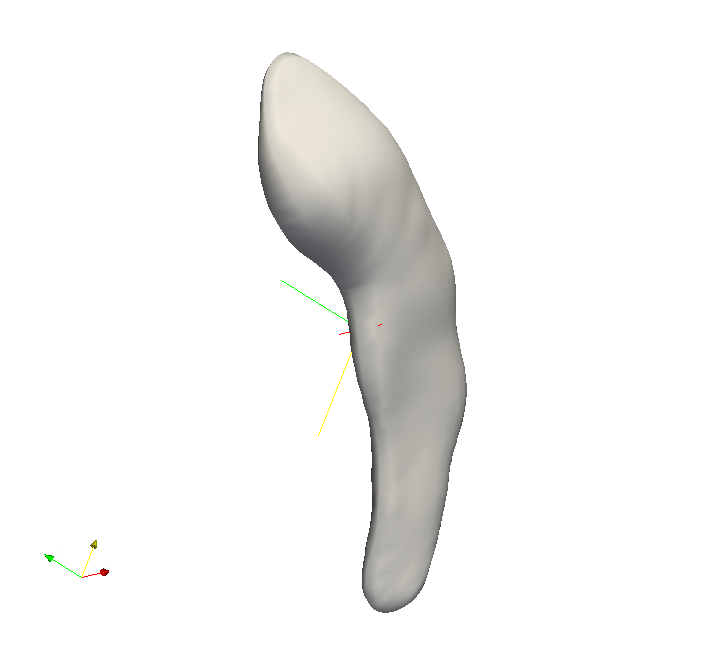
\includegraphics[width=22mm, height=22mm, frame]{./figure/Observation1.png} } \nonumber 
  \hspace{23.2mm}
  \subfloat{ 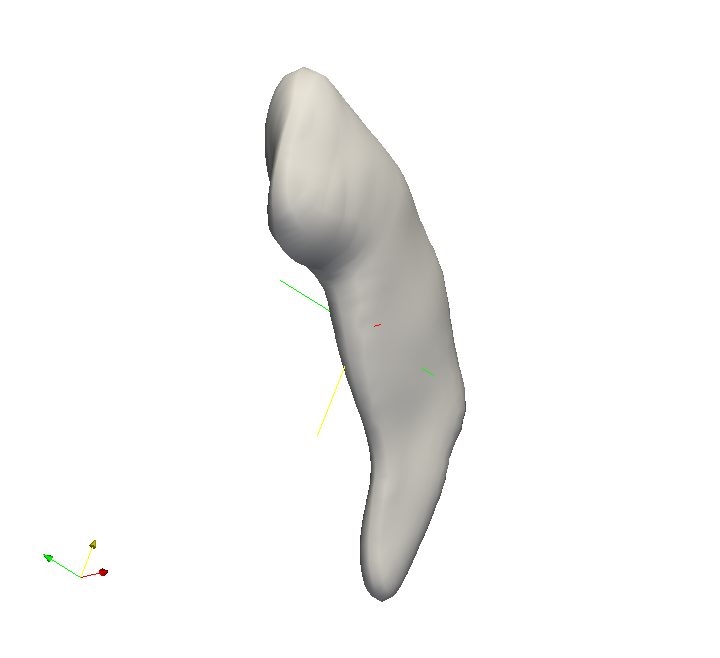
\includegraphics[width=22mm, height=22mm, frame]{./figure/Observation2.png} } \nonumber 
  \hspace{23.4mm}
  \subfloat{ 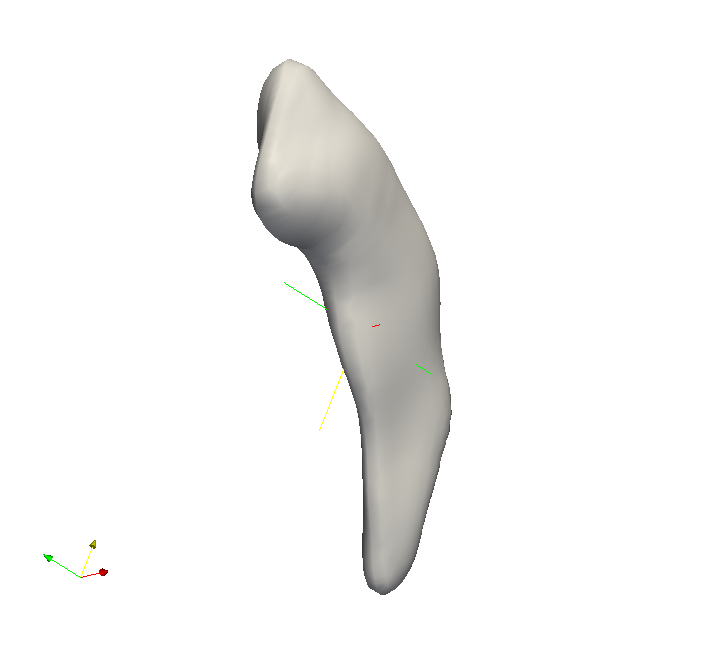
\includegraphics[width=22mm, height=22mm, frame]{./figure/Observation3.png} } \nonumber \\ \vspace{-3mm}
  \subfloat{ 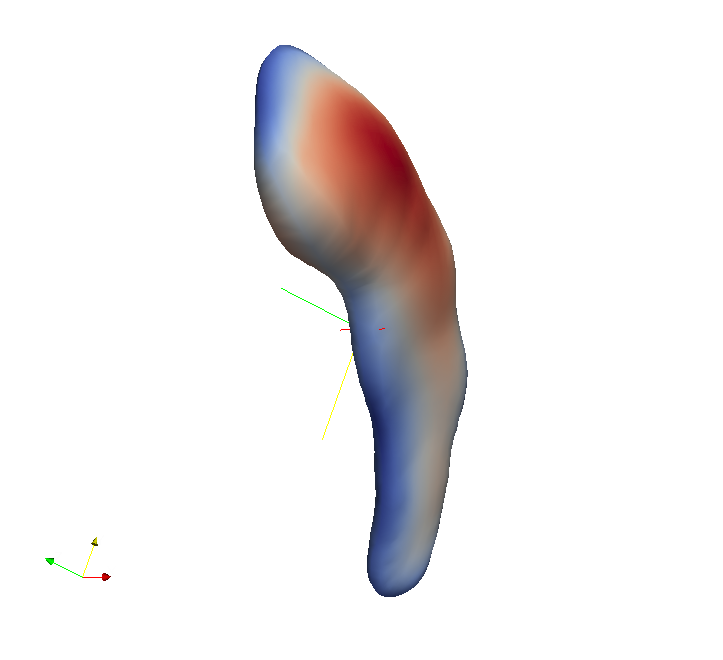
\includegraphics[width=22mm, height=22mm, frame]{./figure/ReconTraj_01.png} } \nonumber 
  \subfloat{ 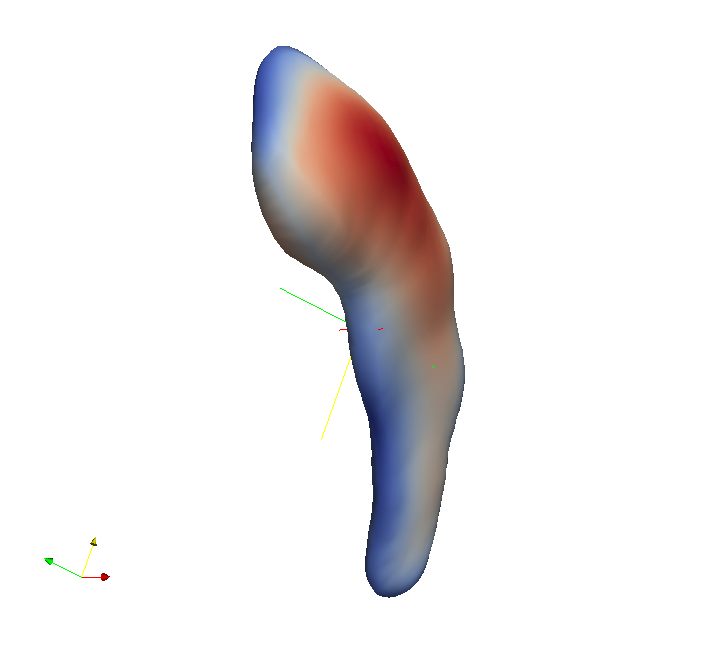
\includegraphics[width=22mm, height=22mm, frame]{./figure/ReconTraj_02.png} } \nonumber 
  \subfloat{ 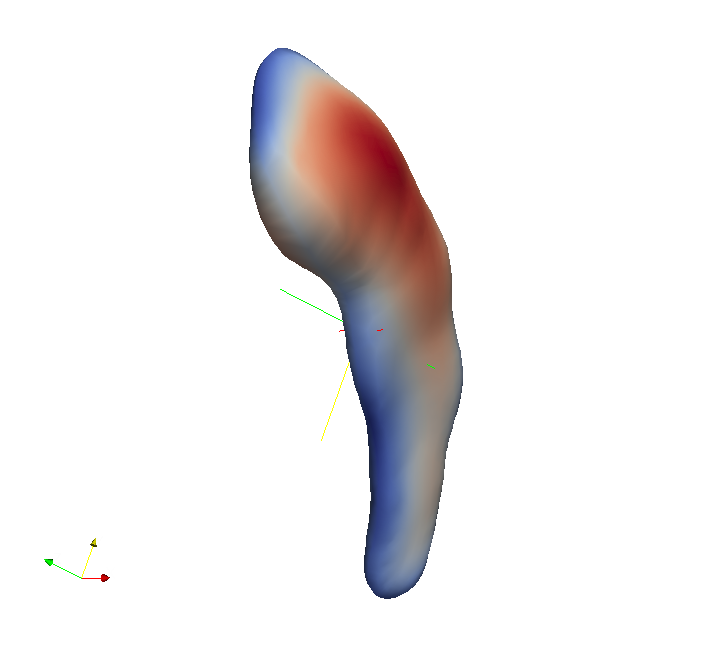
\includegraphics[width=22mm, height=22mm, frame]{./figure/ReconTraj_03.png} } \nonumber 
  \subfloat{ 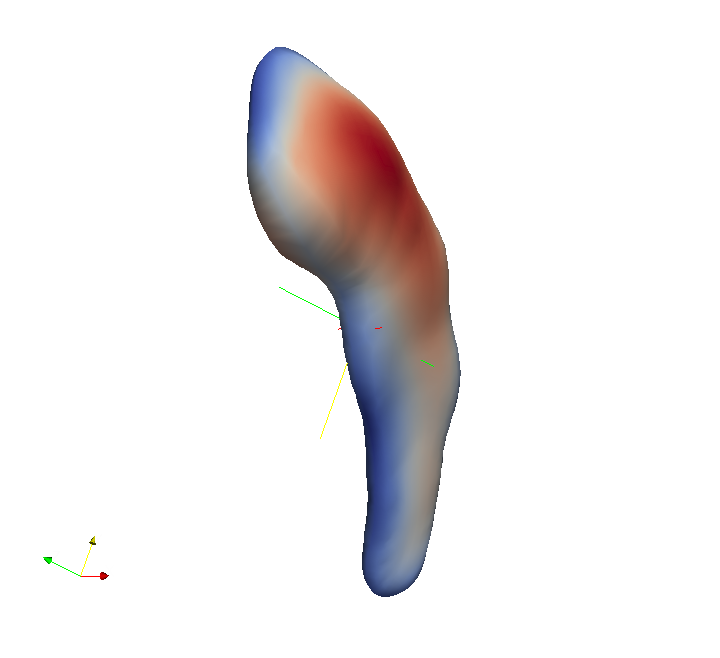
\includegraphics[width=22mm, height=22mm, frame]{./figure/ReconTraj_04.png} } \nonumber 
  \subfloat{ 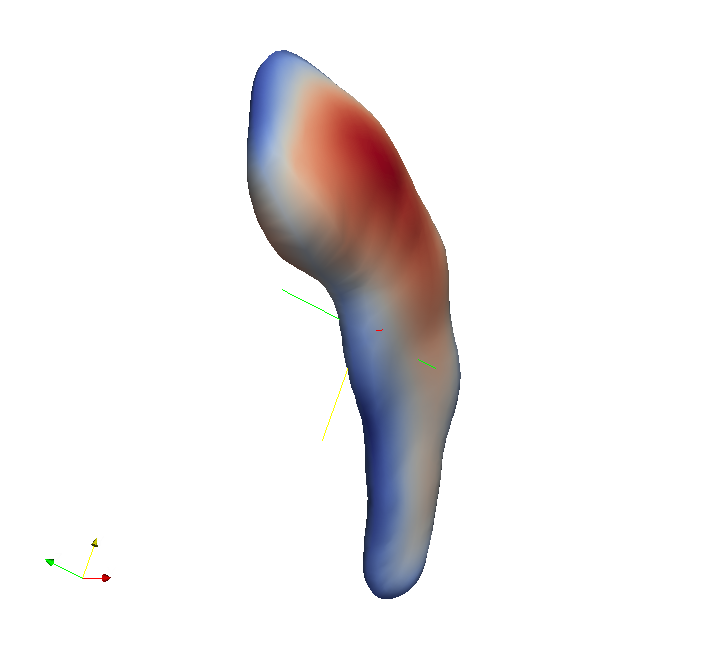
\includegraphics[width=22mm, height=22mm, frame]{./figure/ReconTraj_05.png} } \nonumber \\ \vspace{-3mm}
  \subfloat{ 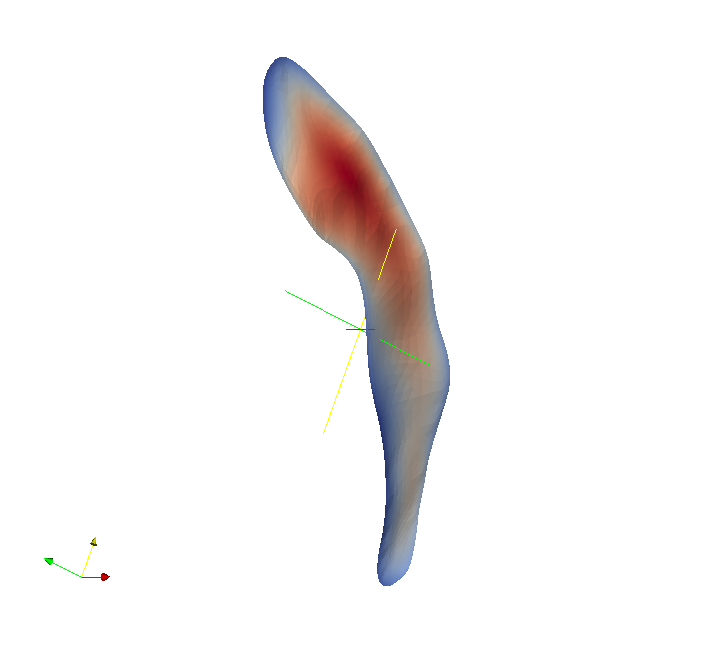
\includegraphics[width=22mm, height=22mm, frame]{./figure/CMRepTraj_01.png} } \nonumber  
  \subfloat{ 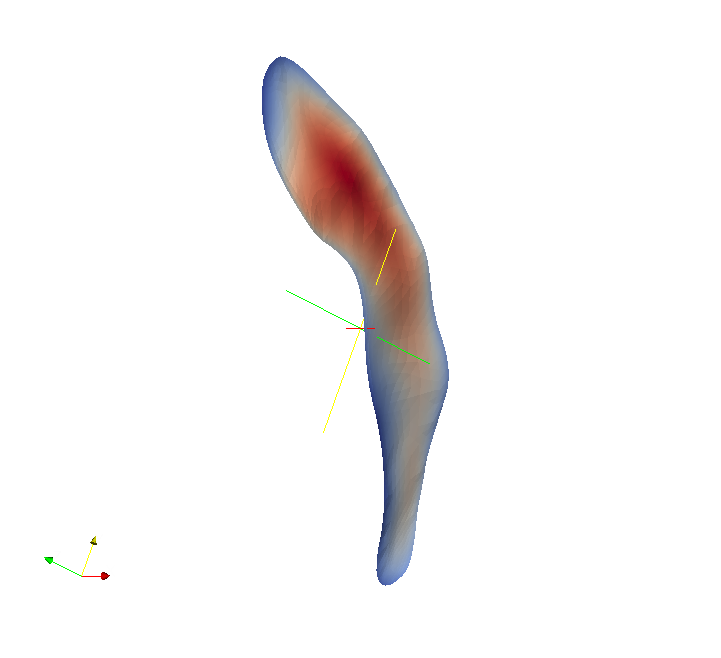
\includegraphics[width=22mm, height=22mm, frame]{./figure/CMRepTraj_02.png} } \nonumber 
  \subfloat{ 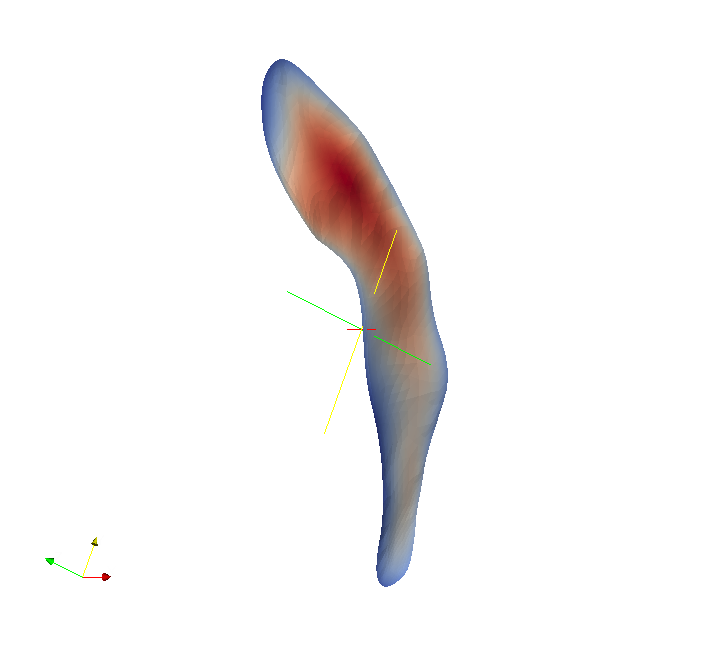
\includegraphics[width=22mm, height=22mm, frame]{./figure/CMRepTraj_03.png} } \nonumber 
  \subfloat{ 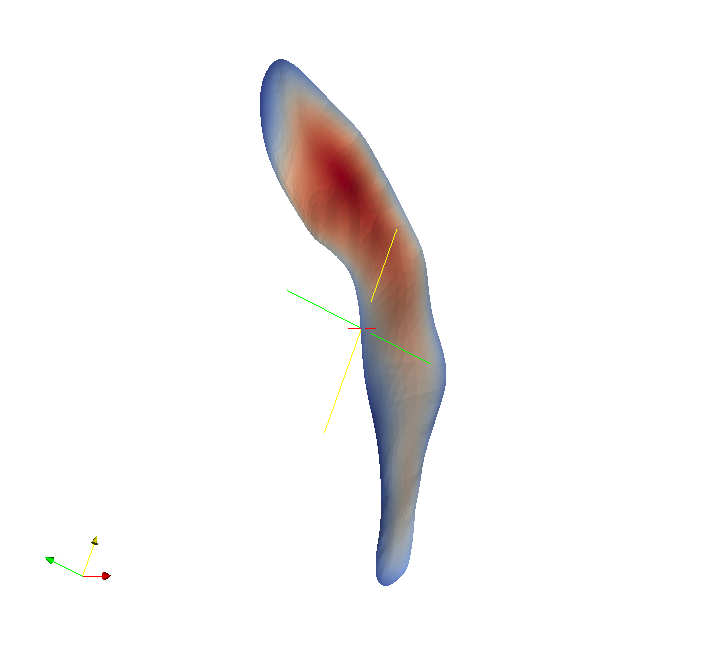
\includegraphics[width=22mm, height=22mm, frame]{./figure/CMRepTraj_04.png} } \nonumber 
  \subfloat{ 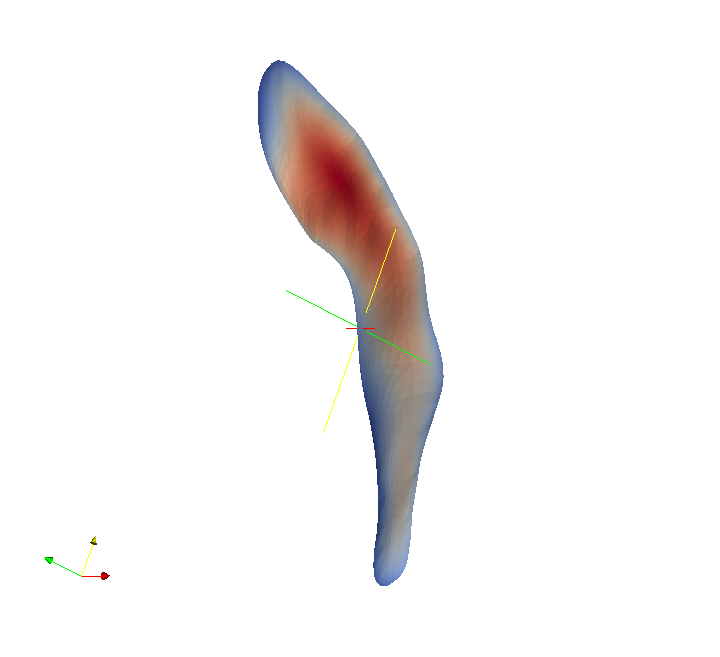
\includegraphics[width=22mm, height=22mm, frame]{./figure/CMRepTraj_05.png} } \nonumber 
\caption{Intermittent observed shapes of a left caudate of a high risk subject (top row), the continuous trajectory of reconstructed shape boundaries (second row) and the continuous trajectory of CM-Reps. Radius scalar fields on both shape boundaries and CM-Reps are color coded to show thick (red) and thin (blue) parts of the estimated shape boundaries}
\label{figTrajs}
\end{figure}


\begin{figure}[htb!]
\centering
  \subfloat[Radius change - High risk]{ 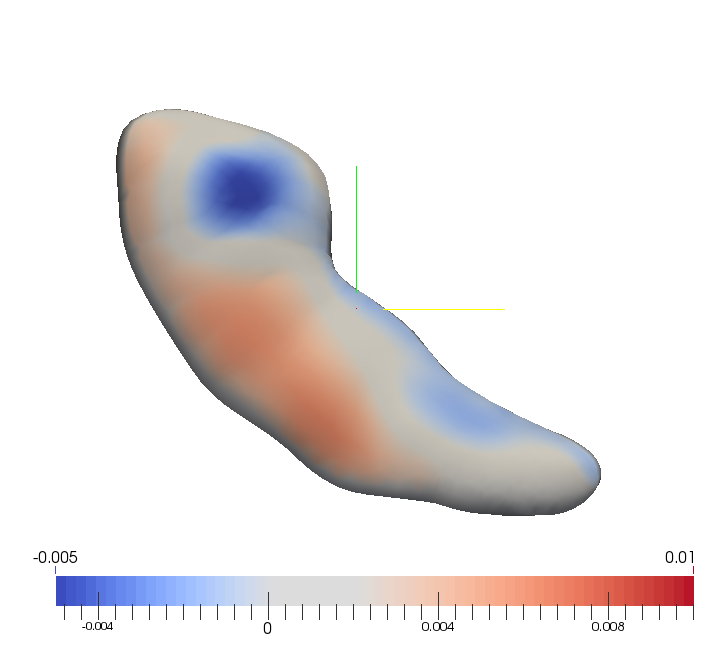
\includegraphics[width=50mm, height=40mm]{./figure/RadiusSlope_High_ColorBar.png} }  
  \subfloat[Radius change - Control]{ 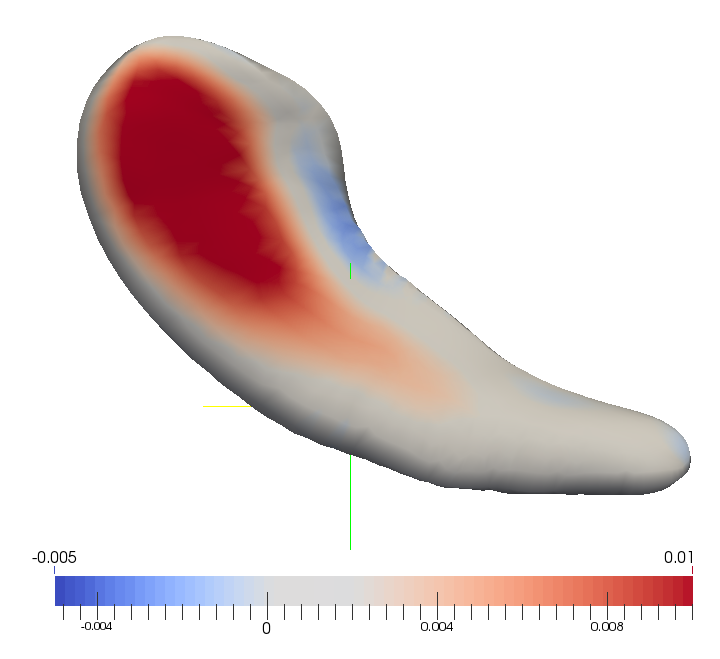
\includegraphics[width=50mm, height=40mm]{./figure/RadiusSlope_Cont_ColorScale.png} } \\
  \subfloat[p value - High risk]{ 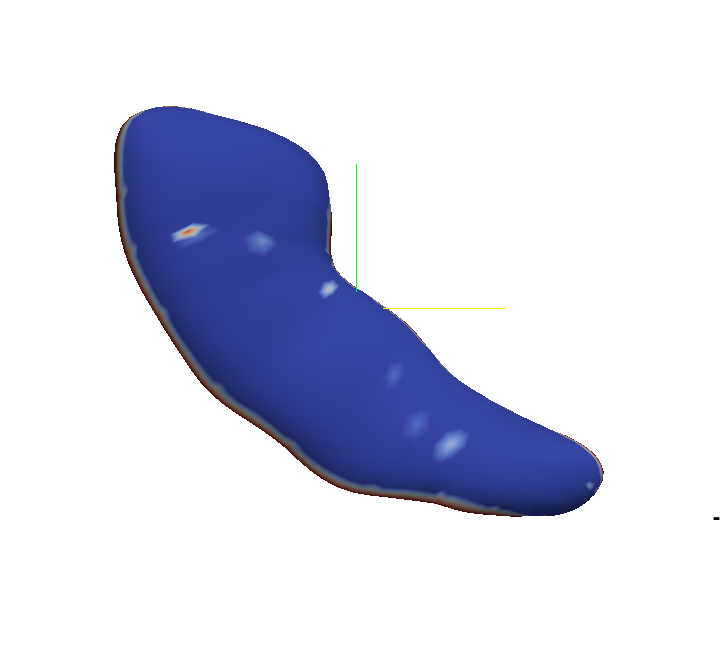
\includegraphics[width=50mm, height=40mm]{./figure/PValue_High.png} } 
  \subfloat[p value - Control]{ 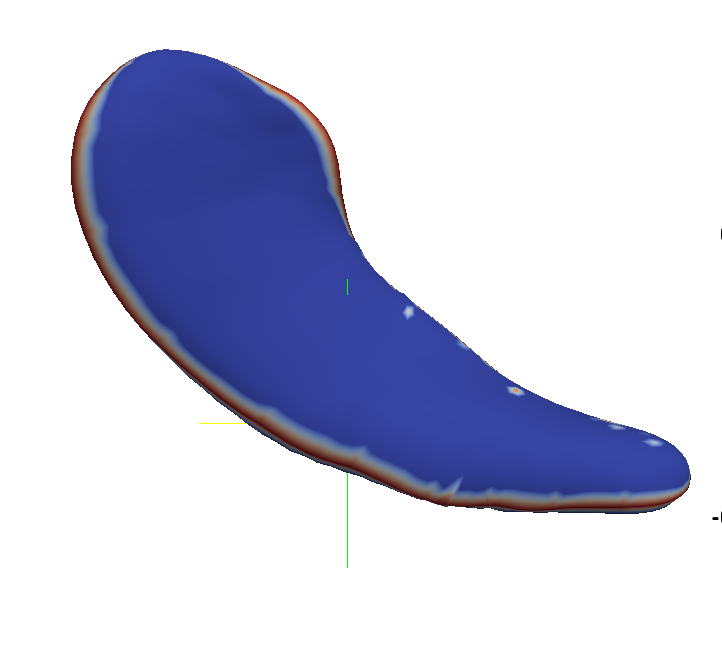
\includegraphics[width=50mm, height=40mm]{./figure/PValue_Cont.png} } 
\caption{ Intial template shape boundaries of a high risk subject and a control group subject color coded with the slope of radius change over time. (a) The subregion of the left caudate of a high risk subject has the selective atrophy which does not appear on (b) the caudate of a control group subject. In (c) and (d), p values with 99\% confidence interval of the estimated slope by linear regression over time at each point is color coded on reconstructed shape surface. }
\label{figRadiusSlope}
\end{figure}

We apply our method to analyze the shape changes of a caudate in basal ganglia compex of a high risk subject and a control group subject from PREDICT-HD Huntinton's disease (HD) database~\cite{Paulsen2014}.
Shape data of caudates of HD patients have interesting features which well suits availability of the proposed method. Each subject has only a few scans, typically two to four scans, with 0.5-2.5 years interval between scans. Since interval periods are varying for each subject and even between scans, the continuous shape trajectories are utmostly necessary to study correlation between shape changes and disease progression. Also, the clinical study~\cite{Vonsattel1985} suggested the selective atrophy of caudates for HD patients, which is not straight forward to be captured by previously suggested shape regression methods. 

Figure~\ref{figTrajs} displays the observed shapes (first row), the trajectory of reconstructed shape boundaries (second row) and the continuous trajectory of CM-Reps (third row) estimated by the proposed method. 
CM-Reps and reconstructed shape boundaries are sampled from continuous trajectories, but a CM-Rep and a shape boundary at any time point within an observation period can be selected by shoot-and-flow diffeomorphisms to an initial baseline CM-Rep and its radius scalar field. The radius scalar field of each shape in trajectories are color coded as thicker parts of a shape with a large radius is displayed as red and blue indicates thinner subregions. The videos of the estimated continuous trajectories of CM-Reps and shape boundaries are included in a supplementary material. 

We analyzed how radius on a reconstructed shape boundary changed over time to show the selective atrophy of caudates for a high risk subject. 
Figure~\ref{figRadiusSlope} shows the radius changes over time on reconstructed shape boundaries at an initial time point for each individual. 
We overlay the rate of radius changes which is the slope of radius change on a shape surface as a color function from blue (negative slope, atrophy) to red (positive slope, expansion). 
The slope is estimated by applying linear regression on radii at each point on a reconstructed shape boundary trajectory over time. 
The bottom row shows the two-sided p value of linear regression at each point for a null hypothesis test on a the slope with 99\% confidence interval, blue is statistically significant while red is not. 
We can observe the selective atrophy in the caudate of a high risk subject while the caudate of a control subject tends to expand at the same subregion. 
It is worthwhile to note that the analysis of the selective atrophy is an intuitive application of our method since the correspondence between CM-Reps and reconstructed boundary shapes are naturally established in our framework. 



\begin{comment}
\begin{figure}[htb!]
\centering
  \subfloat{ 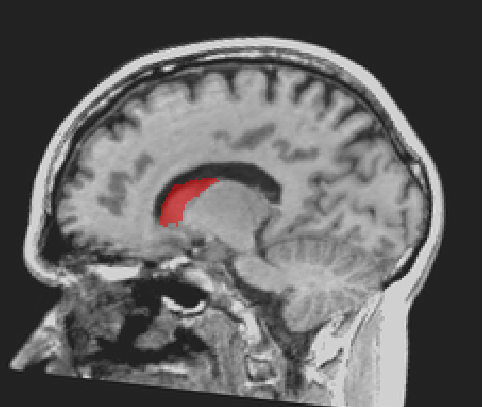
\includegraphics[width=33mm, height=33mm]{./figure/lc_seg_00.png} } \nonumber \hfill 
  \subfloat{ 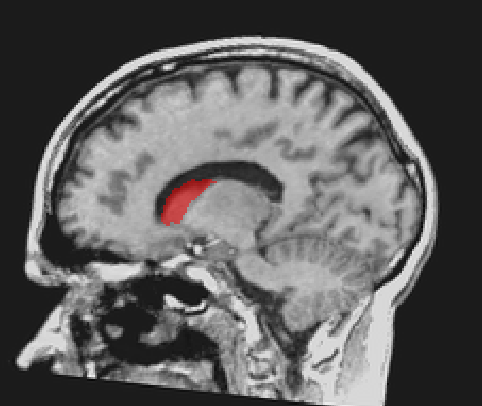
\includegraphics[width=33mm, height=33mm]{./figure/lc_seg_01.png} } \nonumber \hfill 
  \subfloat{ 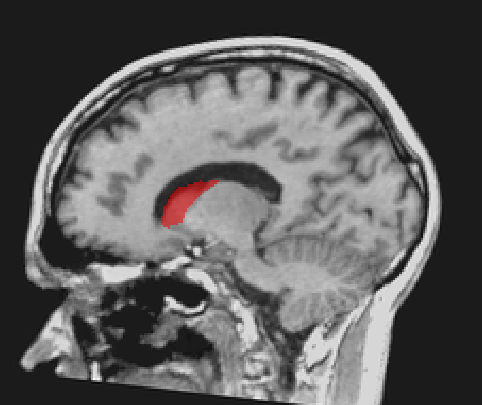
\includegraphics[width=33mm, height=33mm]{./figure/lc_seg_02.png} } \nonumber \hfill 
\caption{d.}
\label{figSegLabels}
\end{figure}
\end{comment}


\section{Conclusions}

\begin{comment}
In this study, we proposed a novel framework that makes use of subject-specific shape deformation trajectories by diffeomorphic shape regression models and the longitudinal statistical analysis.
Results show how the shape deformation has more significance than the volumetric analysis and how significantly it correlates with continuous CAP score for a global shape and local subregions. 
The global shape analysis showed that the gradient magnitude of deformation vectors over global shape has better significance than volume-wise metric regardless of different baseline shapes of different subjects.
The local shape analysis also revealed statistically significant general trends of subregion shape changes. 
As a future direction, the analysis will also be extended to develop an HD progression model that will allow prediction of the stage of disease of individuals based on shape biomarkers.
\end{comment}

\bibliography{MICCAI2017.bib}
\bibliographystyle{splncs03}



\end{document}
